\qns{An Introduction to Bode Plots}
\qcontributor{Justin Yu, Taejin Hwang}

[Add intro here...]

% \begin{center}
% 		\begin{circuitikz}[scale=0.8]
% 			\draw (0,4)
% 			to [sV, l_= $\tilde{V_s}$] (0,0)
% 			(0,4)
% 			to [R = $R$,v=$\tilde{V_R}$] (4,4)
% 			to [L = $L$,v=$\tilde{V_L}$] (8,4)
% 			to [short] (10,4)
% 			to [C = $C$,v=$\tilde{V_C}$] (10,0)
% 			to [short] (0,0);
% 		\end{circuitikz}
% 	\end{center}

\begin{enumerate}

\qitem Let's start by taking a look at $H(\omega) = X(\omega)Y(\omega)$, the product of two transfer functions $X$ and $Y$.
\begin{enumerate}
    \qitem How can you graph $|H(\omega)|$ using the graphs of $|X(\omega)|$, $|Y(\omega)|$?
    \qitem How does this compare when graphing ...
\end{enumerate}

\sol{
}

We made note in the previous question that any transfer function can be written in its \textit{ational transfer function form.}
We'll now look at four fundamental Bode plots that make up this form.

\qitem Let $H_z(\omega) = 1 + j \frac{\omega}{\omega_z}$. This is called a \textbf{zero at $\omega_z$}, where $\omega_z$ is the \textbf{zero frequency}.
\begin{enumerate}
    \qitem \textbf{Find $|H_z(\omega)|$ and $\angle H_z(\omega)$.}
           \textit{Hint: Consider the geometric interpretation of the transfer function as a complex number.
           Calculating the magnitude and angle is the same as in standard Cartesian coordinates.}
    \qitem Bode plots are approximations to the true transfer function, which means we only need to analyze the behavior in a few regions to sketch out an approximation to any transfer function's behavior.
    Typically, we will analyze the behavior at three regions: $\omega << \omega_z$, $\omega = \omega_z$, and $\omega >> \omega_z$.
    \textbf{Fill in the following table for the values of $H_z(\omega)|$, $|H_z(\omega)|$, $\angle H_z(\omega)$ at these regions:}

    \begin{table}[ht!]
      \centering
      \begin{tabular}{| l | >{\centering\arraybackslash}m{6em} | >{\centering\arraybackslash}m{6em} | >{\centering\arraybackslash}m{6em} |} 
      \cline{2-4}
      \multicolumn{1}{l|}{}& $\omega << \omega_z$ & $\omega = \omega_z$ & $\omega >> \omega_z$ \\
      \hline
      &&&\\
      $H_z(\omega)$        &                      &                     &                      \\
      &&&\\
      \hline
      &&&\\
      $|H_z(\omega)|$      &                      &                     &                      \\
      &&&\\
      \hline
      &&&\\
      $\angle H_z(\omega)$ &                      &                     &                      \\
      &&&\\
      \hline
      \end{tabular}
    \end{table}

    \qitem \textbf{Plot the Bode plot for $|H_z(\omega)|$ and $\angle H_z(\omega)$ using the log-log plots below with $\omega$ on the x-axis.} (\textit{Sanity check: Why are we using log-log plots?})

    \begin{quote}
    \textbf{Note:} To plot these log-log plots using the values we calculated in the table above, we approximate the point $\omega << \omega_z$
    to be at $\omega = \frac{\omega_z}{10}$ and the point $\omega >> \omega_z$ to be at $\omega = 10\omega_z$.
    These differ from the zero frequency by a factor of 10 because we are using a base 10 log-log plot. \textbf{Plot the 3 points calculated above and connect them with straight line approximations.}
    \end{quote}

\end{enumerate}

\begin{figure}[!ht]
  \centering
  \begin{minipage}[b]{0.45\textwidth}
  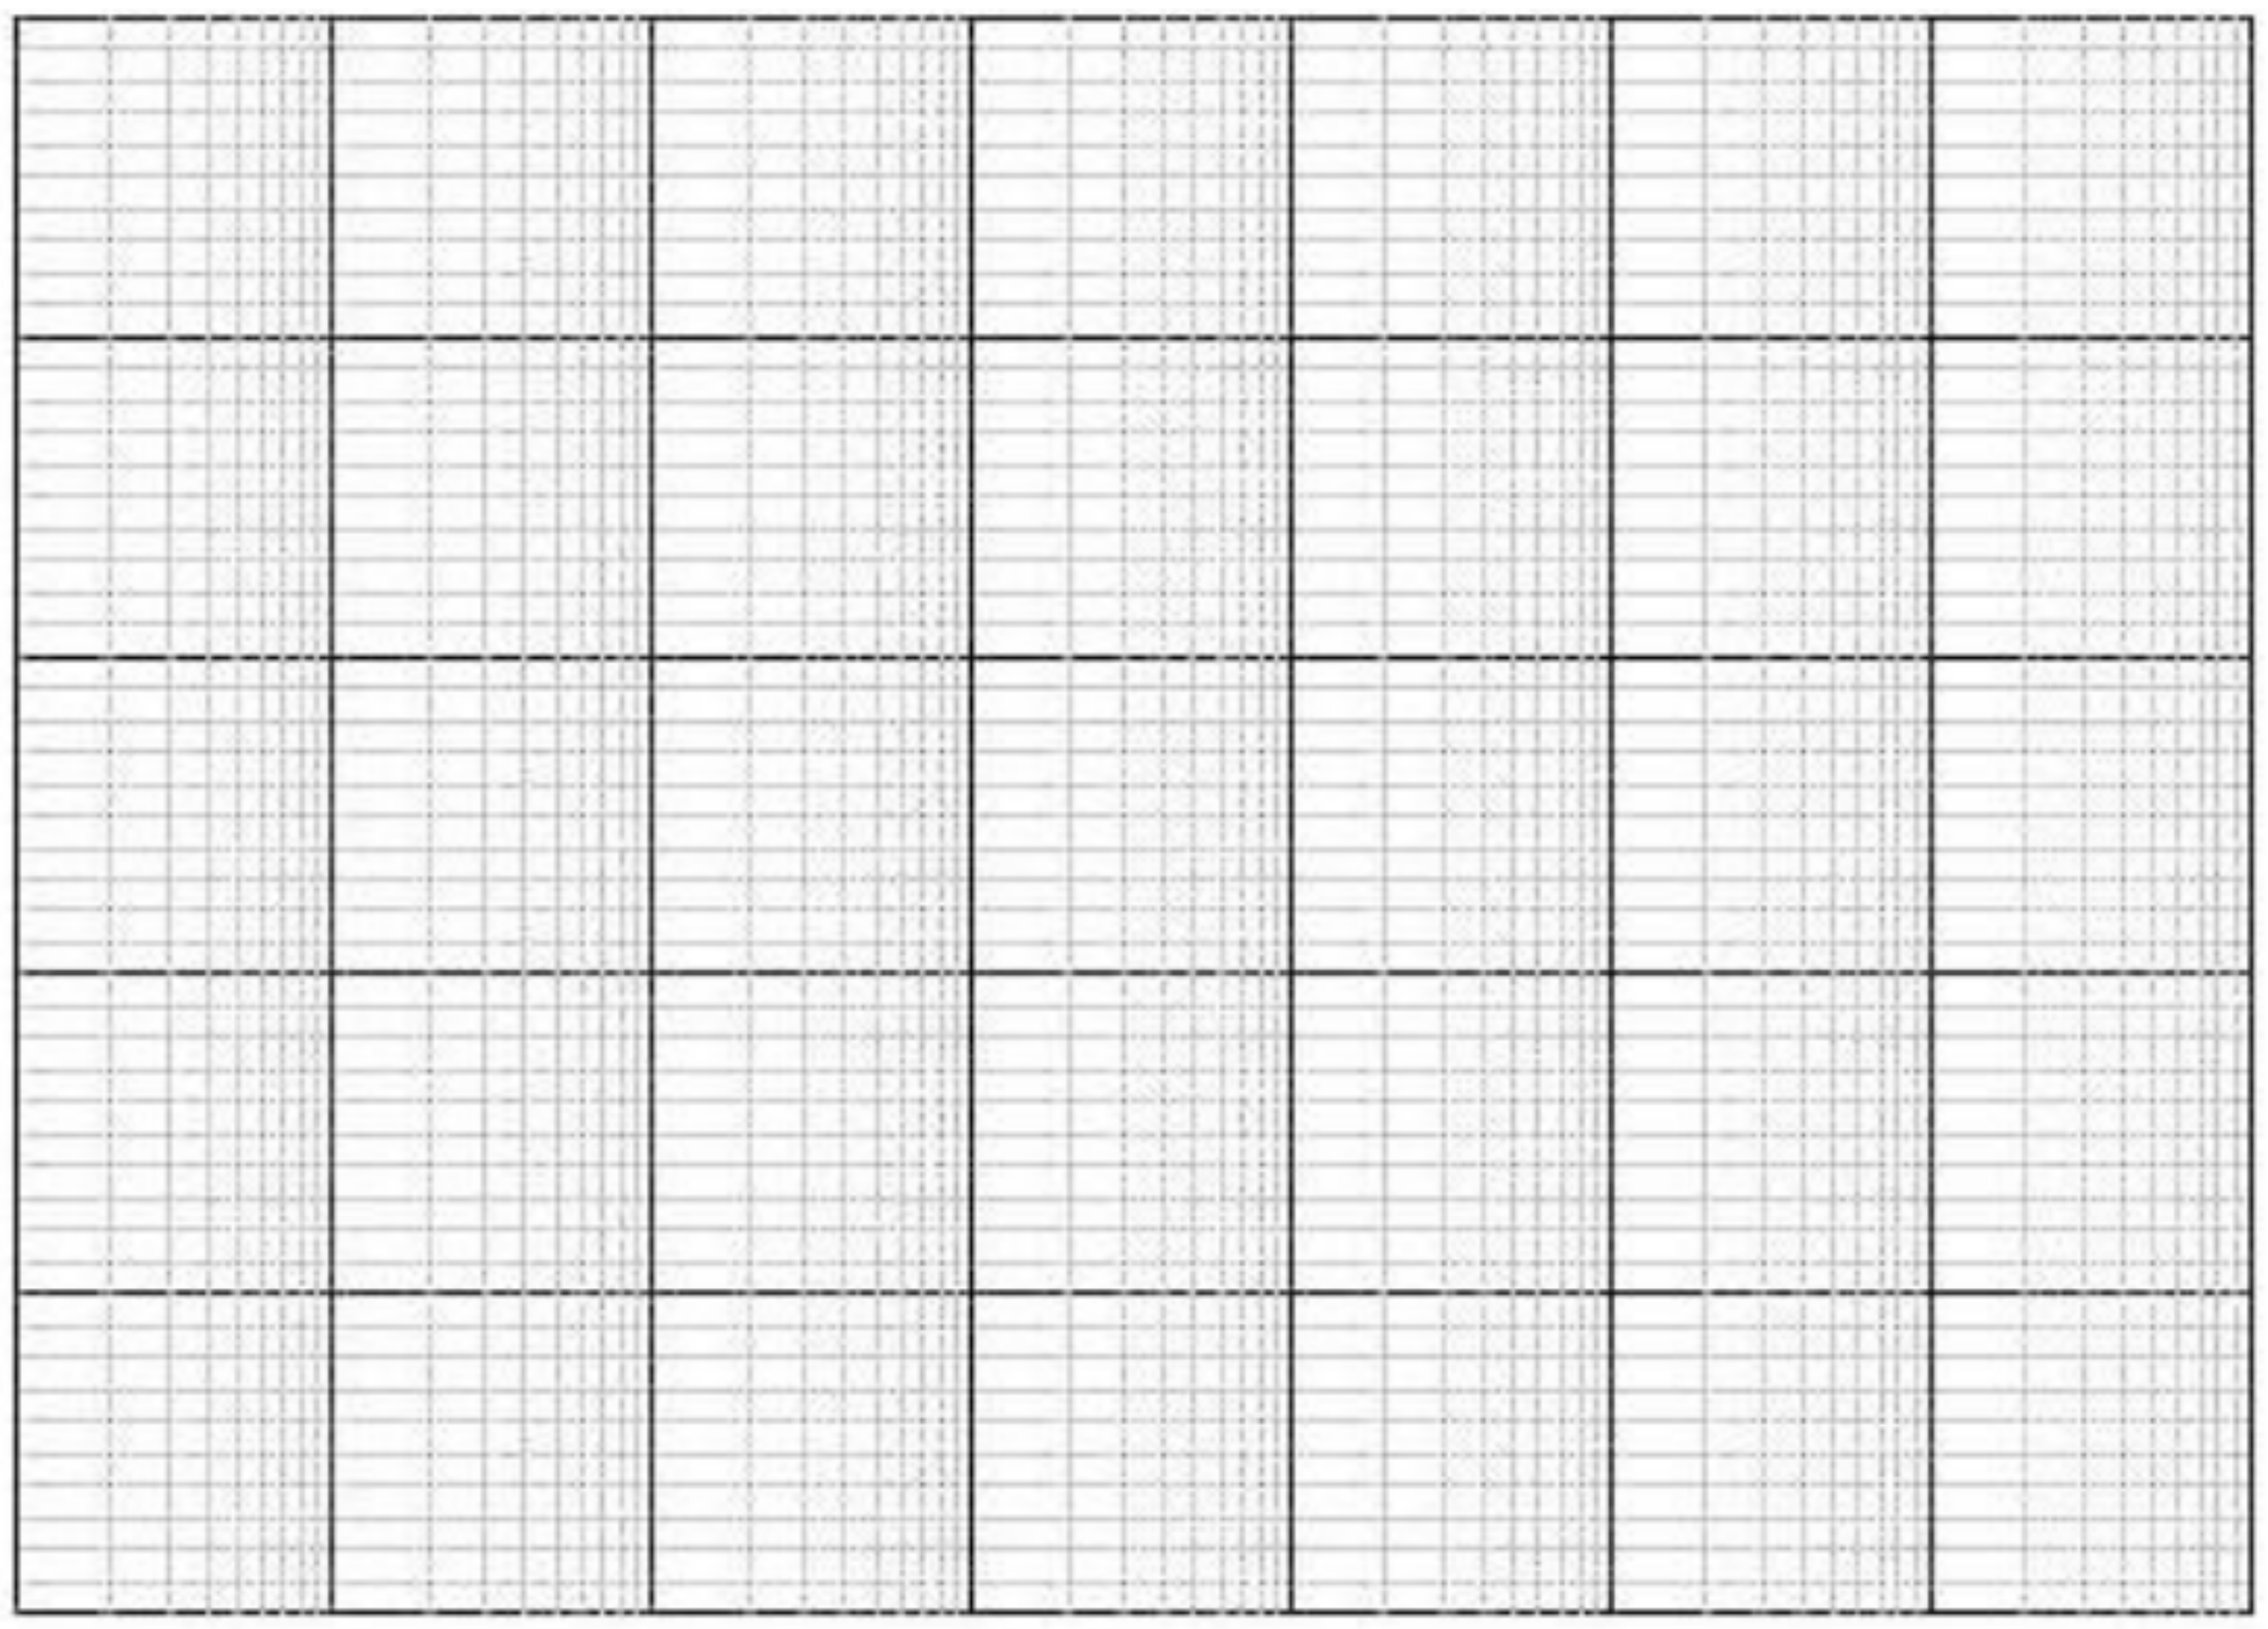
\includegraphics[width=1.0\textwidth]{\bank/transfer/figures/bodeblank}
    \caption*{$|H_z(\omega)|$}
  \end{minipage}
  \hfill
  \begin{minipage}[b]{0.45\textwidth}
  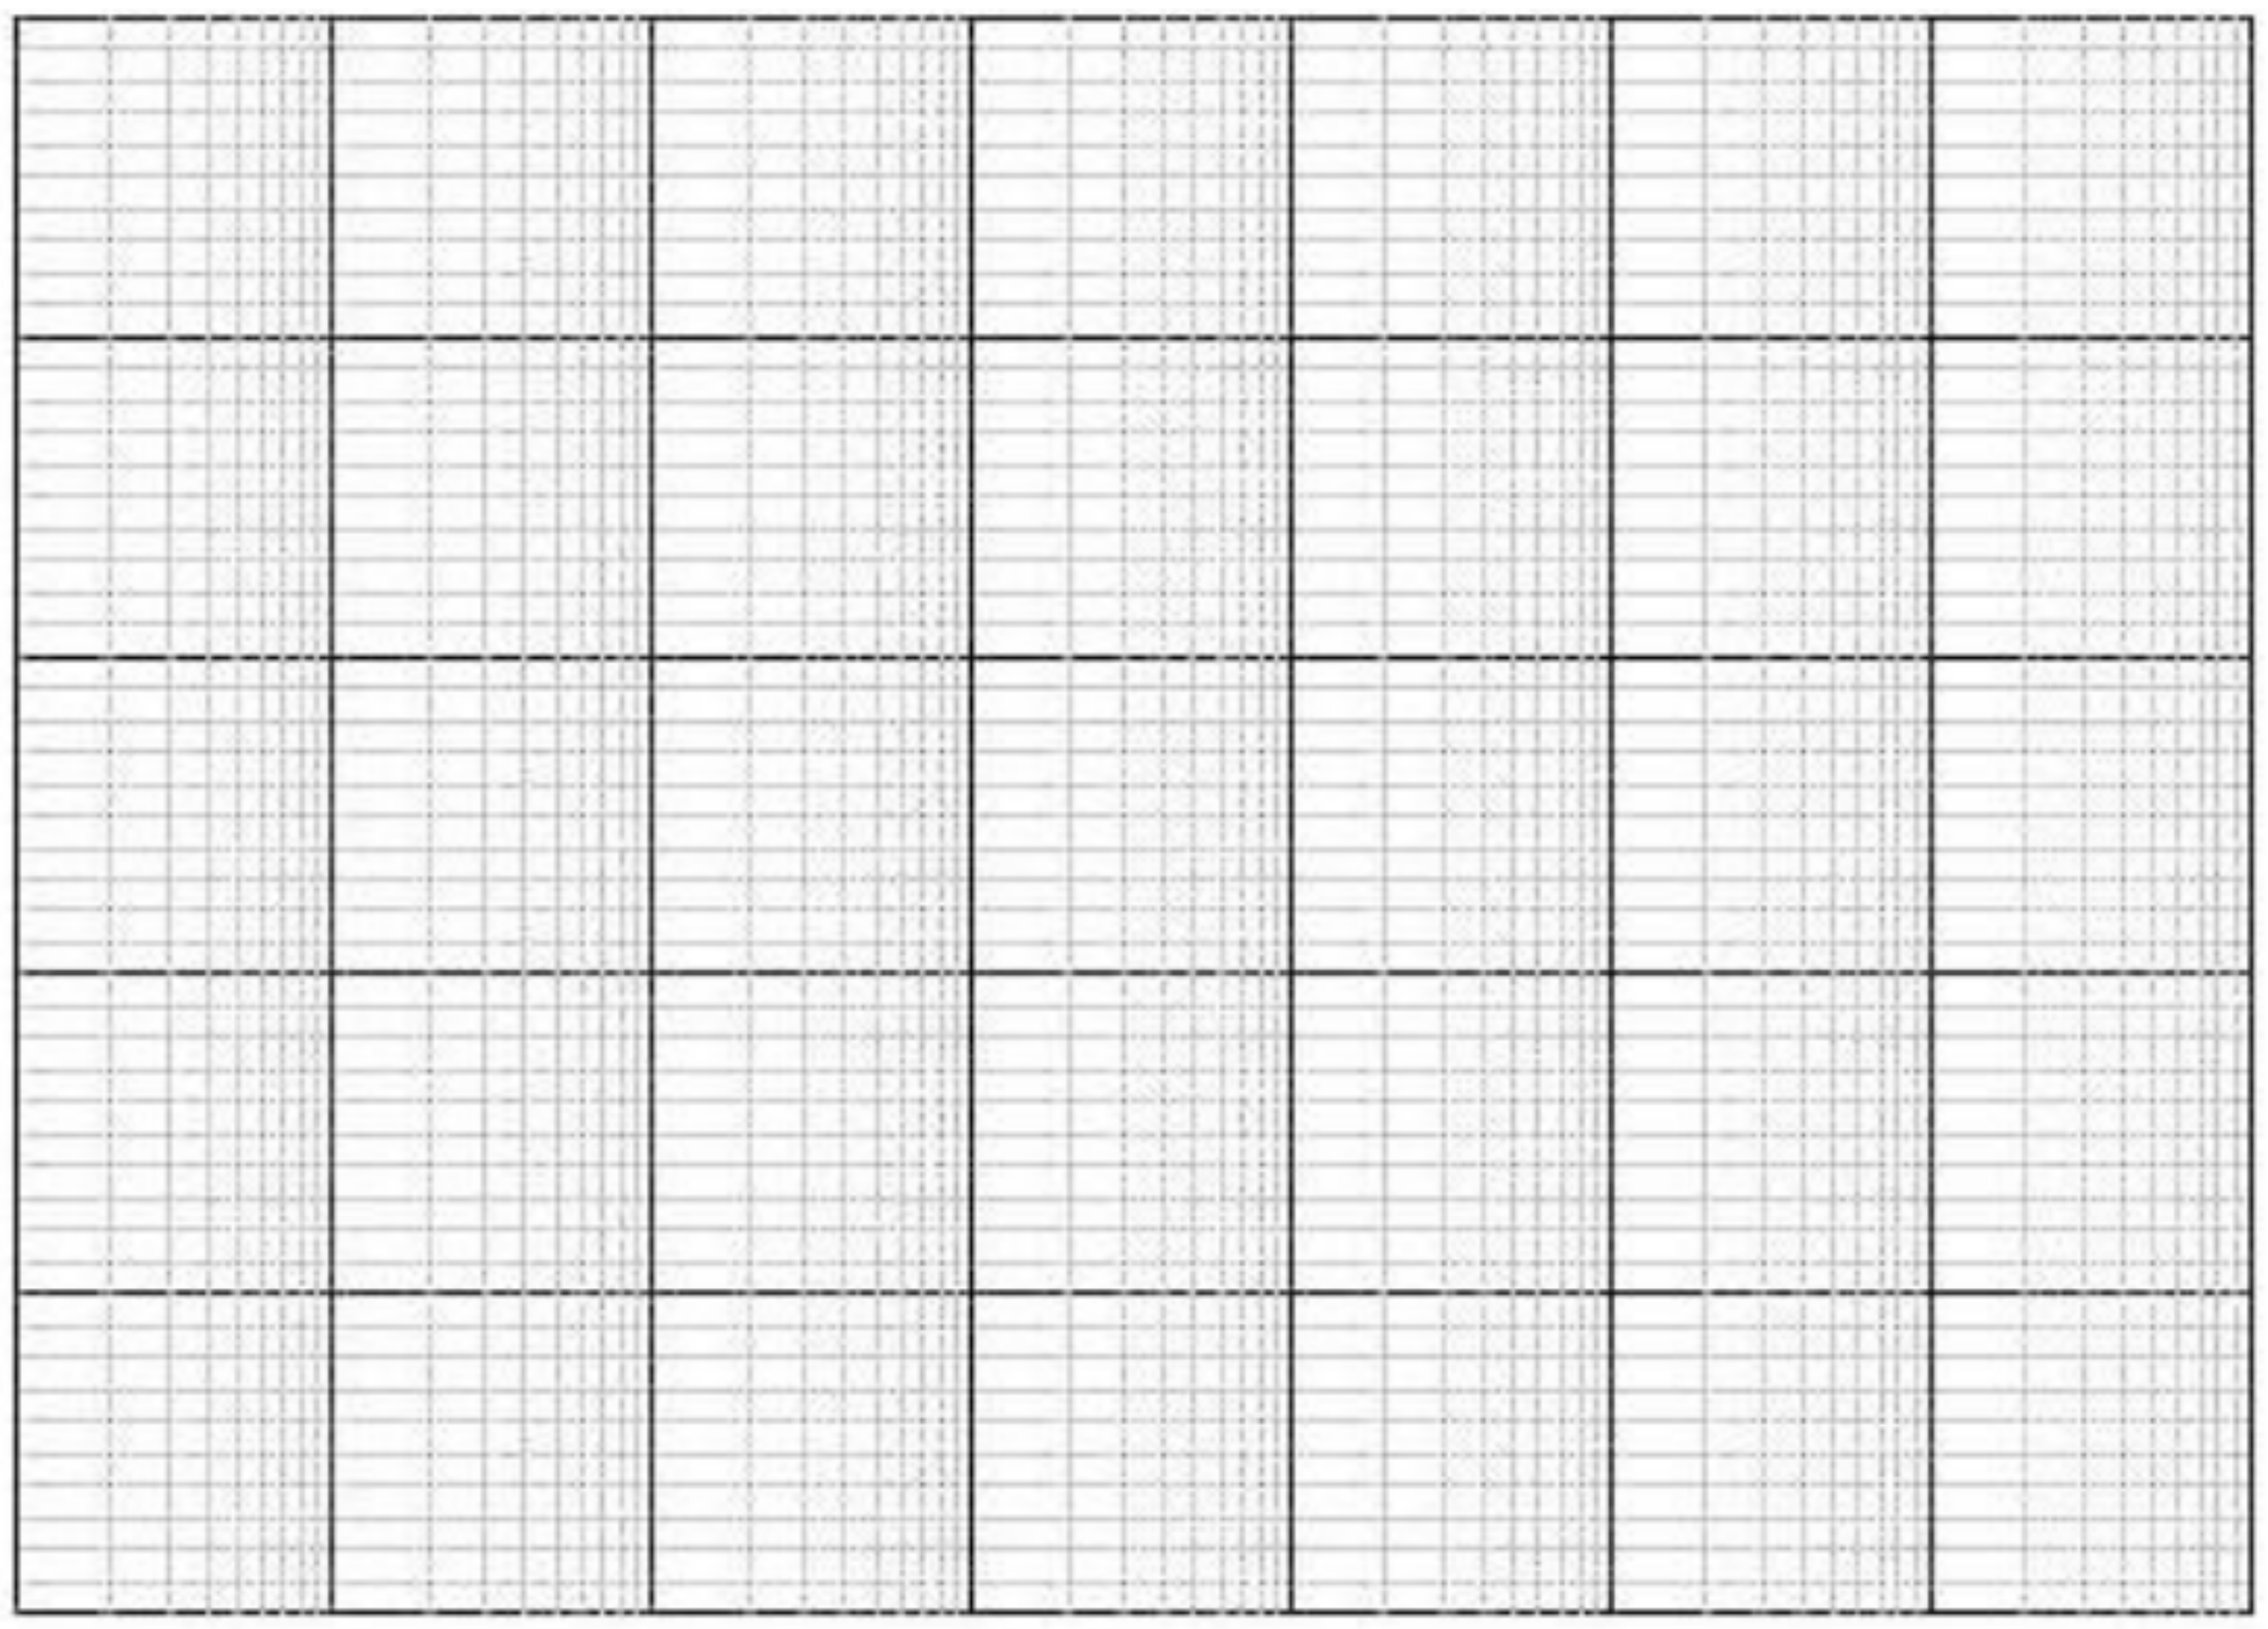
\includegraphics[width=1.0\textwidth]{\bank/transfer/figures/bodeblank}
    \caption*{$\angle H_z(\omega)$}
  \end{minipage}
\end{figure}

\sol{
}

\qitem Let $H_p(\omega) = \frac{1}{1 + j \frac{\omega}{\omega_p}}$. This is called a \textbf{pole at $\omega_p$}, where $\omega_p$ is the \textbf{pole frequency}. Note that this is the reciprocal of the zero in the previous part.
\begin{enumerate}
    \qitem Find $|H_p(\omega)|$ and $\angle H_p(\omega)$.
    \qitem Again, \textbf{fill in the following table to analyze the magnitude and phase at the three regions $\omega << \omega_p$, $\omega = \omega_p$, and $\omega >> \omega_p$.}

    \begin{table}[ht!]
      \centering
      \begin{tabular}{| l | >{\centering\arraybackslash}m{6em} | >{\centering\arraybackslash}m{6em} | >{\centering\arraybackslash}m{6em} |} 
      \cline{2-4}
      \multicolumn{1}{l|}{}& $\omega << \omega_p$ & $\omega = \omega_p$ & $\omega >> \omega_p$ \\
      \hline
      &&&\\
      $H_p(\omega)$        &                      &                     &                      \\
      &&&\\
      \hline
      &&&\\
      $|H_p(\omega)|$      &                      &                     &                      \\
      &&&\\
      \hline
      &&&\\
      $\angle H_p(\omega)$ &                      &                     &                      \\
      &&&\\
      \hline
      \end{tabular}
    \end{table}

    \qitem \textbf{Plot the Bode plot for $|H_p(\omega)|$ and $\angle H_p(\omega)$.}
           Use the same way of approximating as described in the previous part.
\end{enumerate}

\begin{figure}[!ht]
  \centering
  \begin{minipage}[b]{0.45\textwidth}
  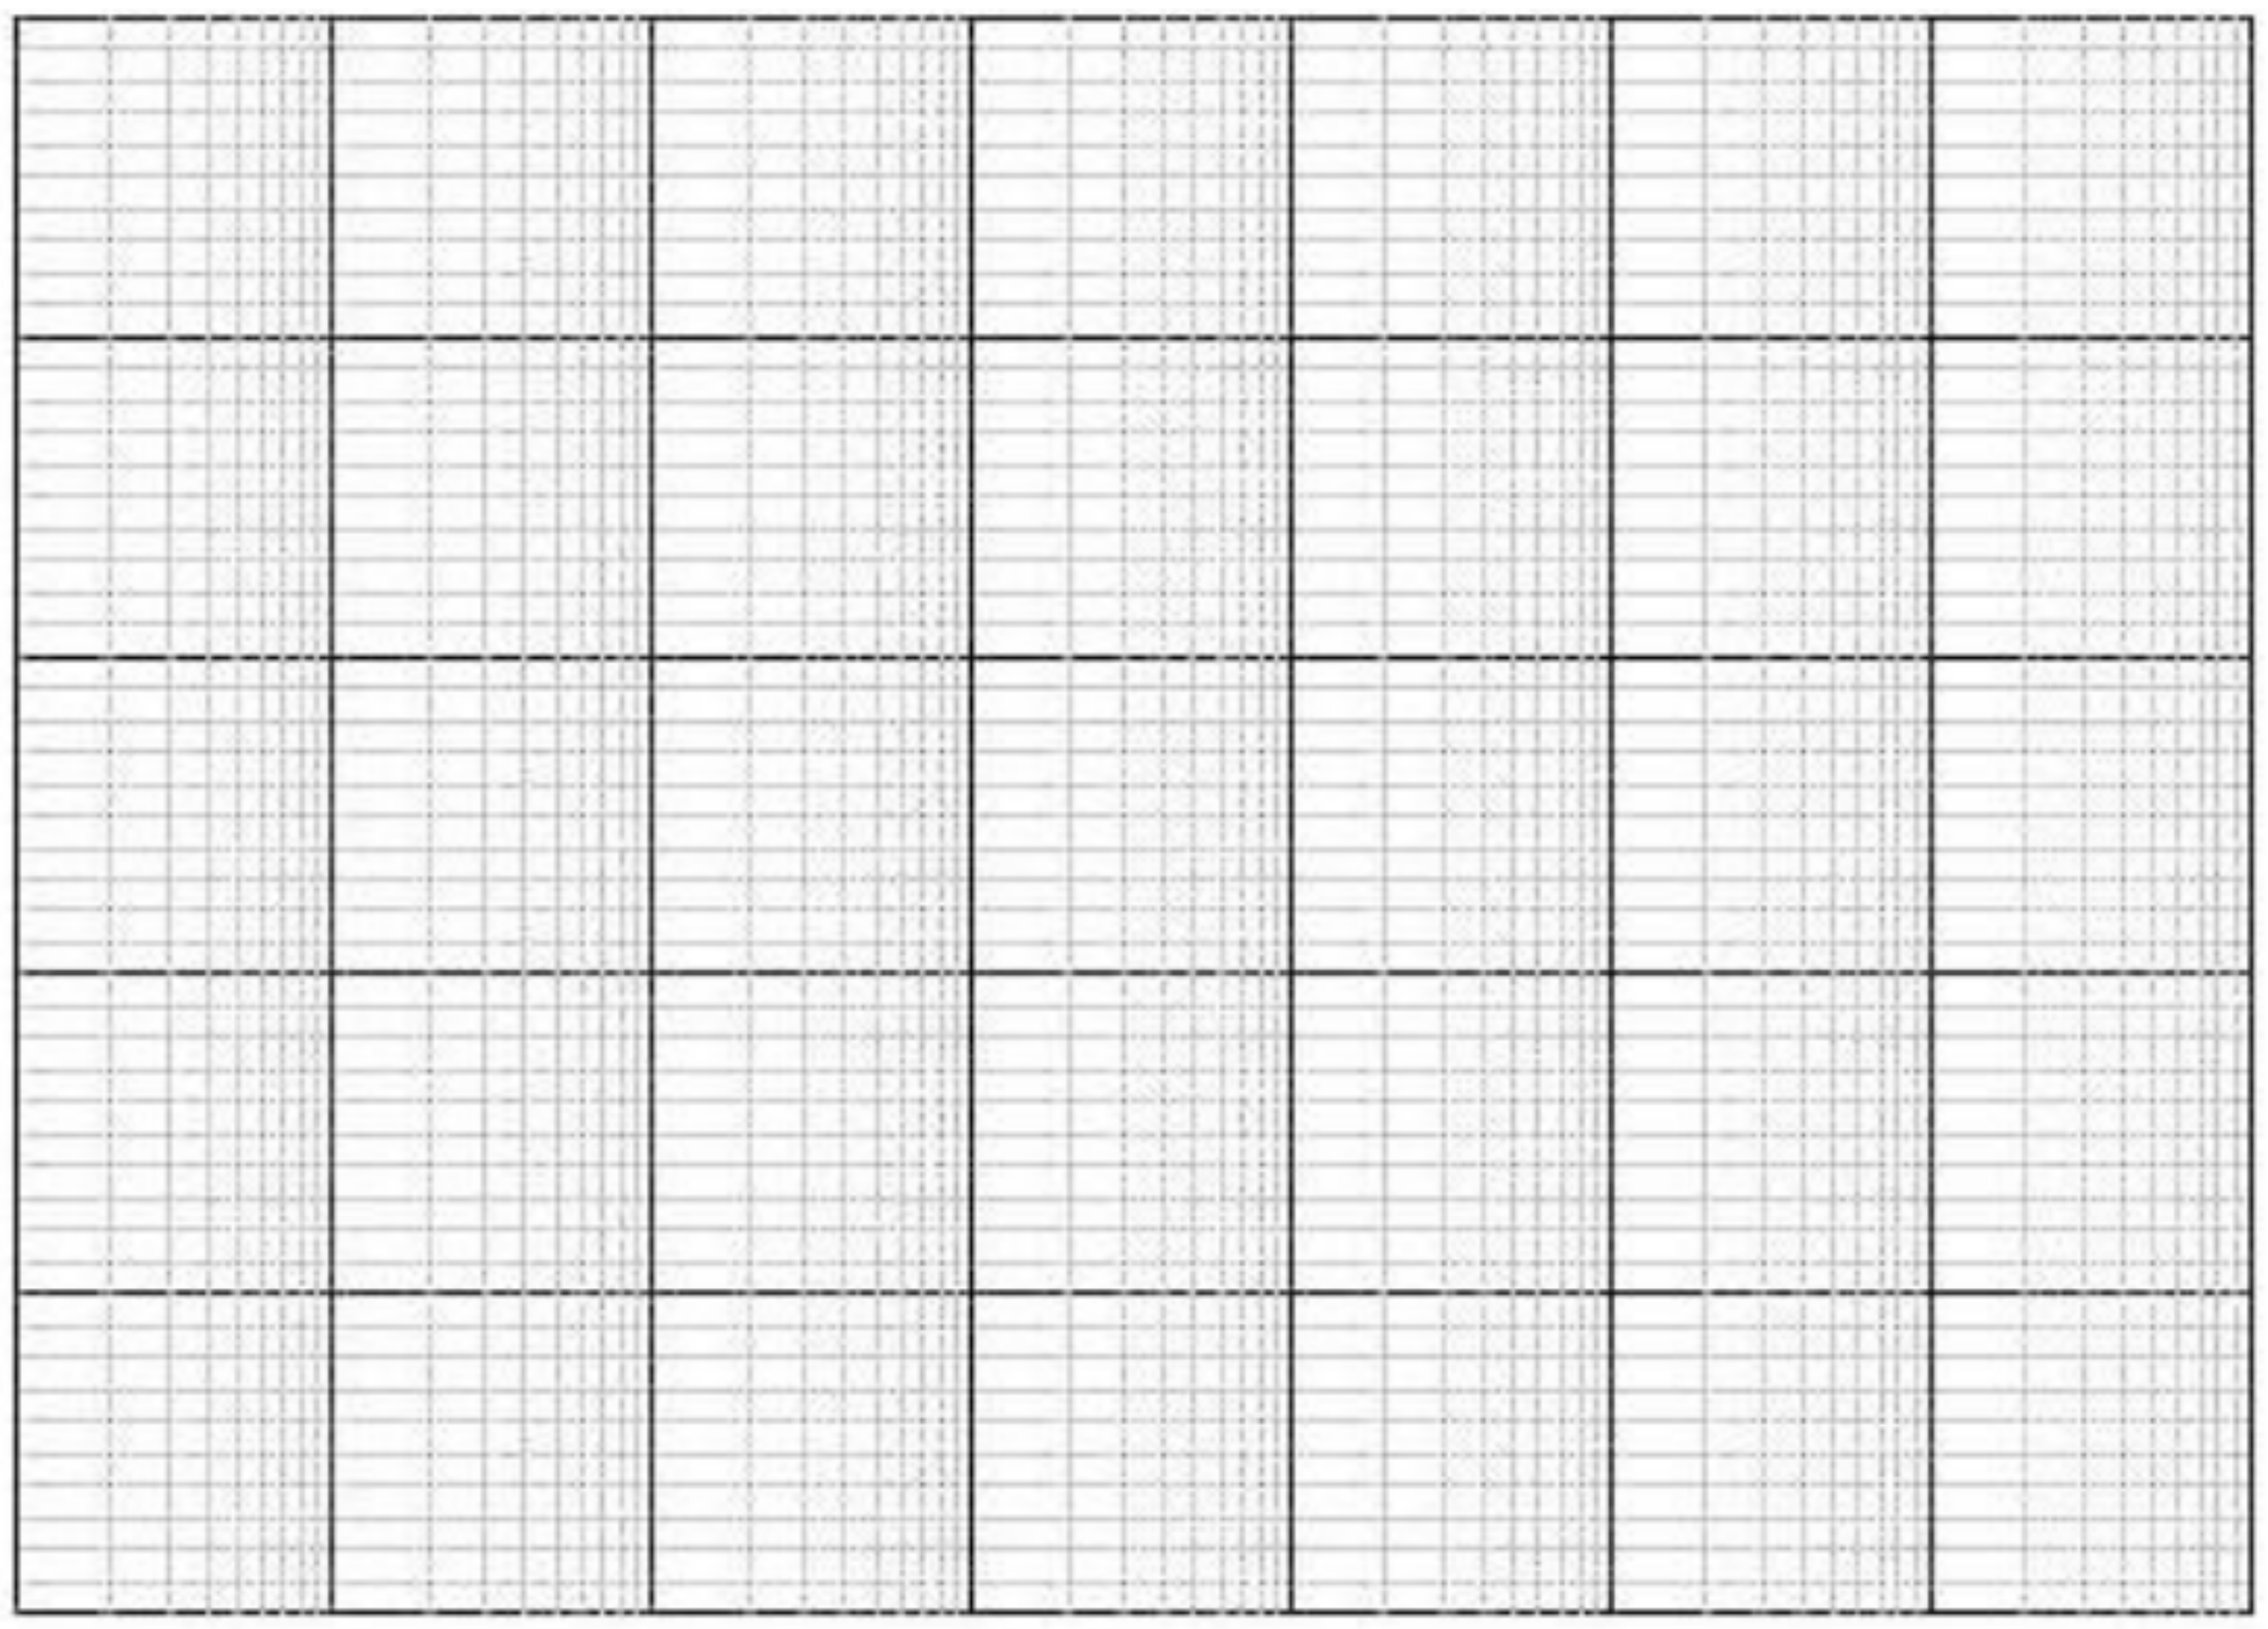
\includegraphics[width=1.0\textwidth]{\bank/transfer/figures/bodeblank}
    \caption*{$|H_z(\omega)|$}
  \end{minipage}
  \hfill
  \begin{minipage}[b]{0.45\textwidth}
  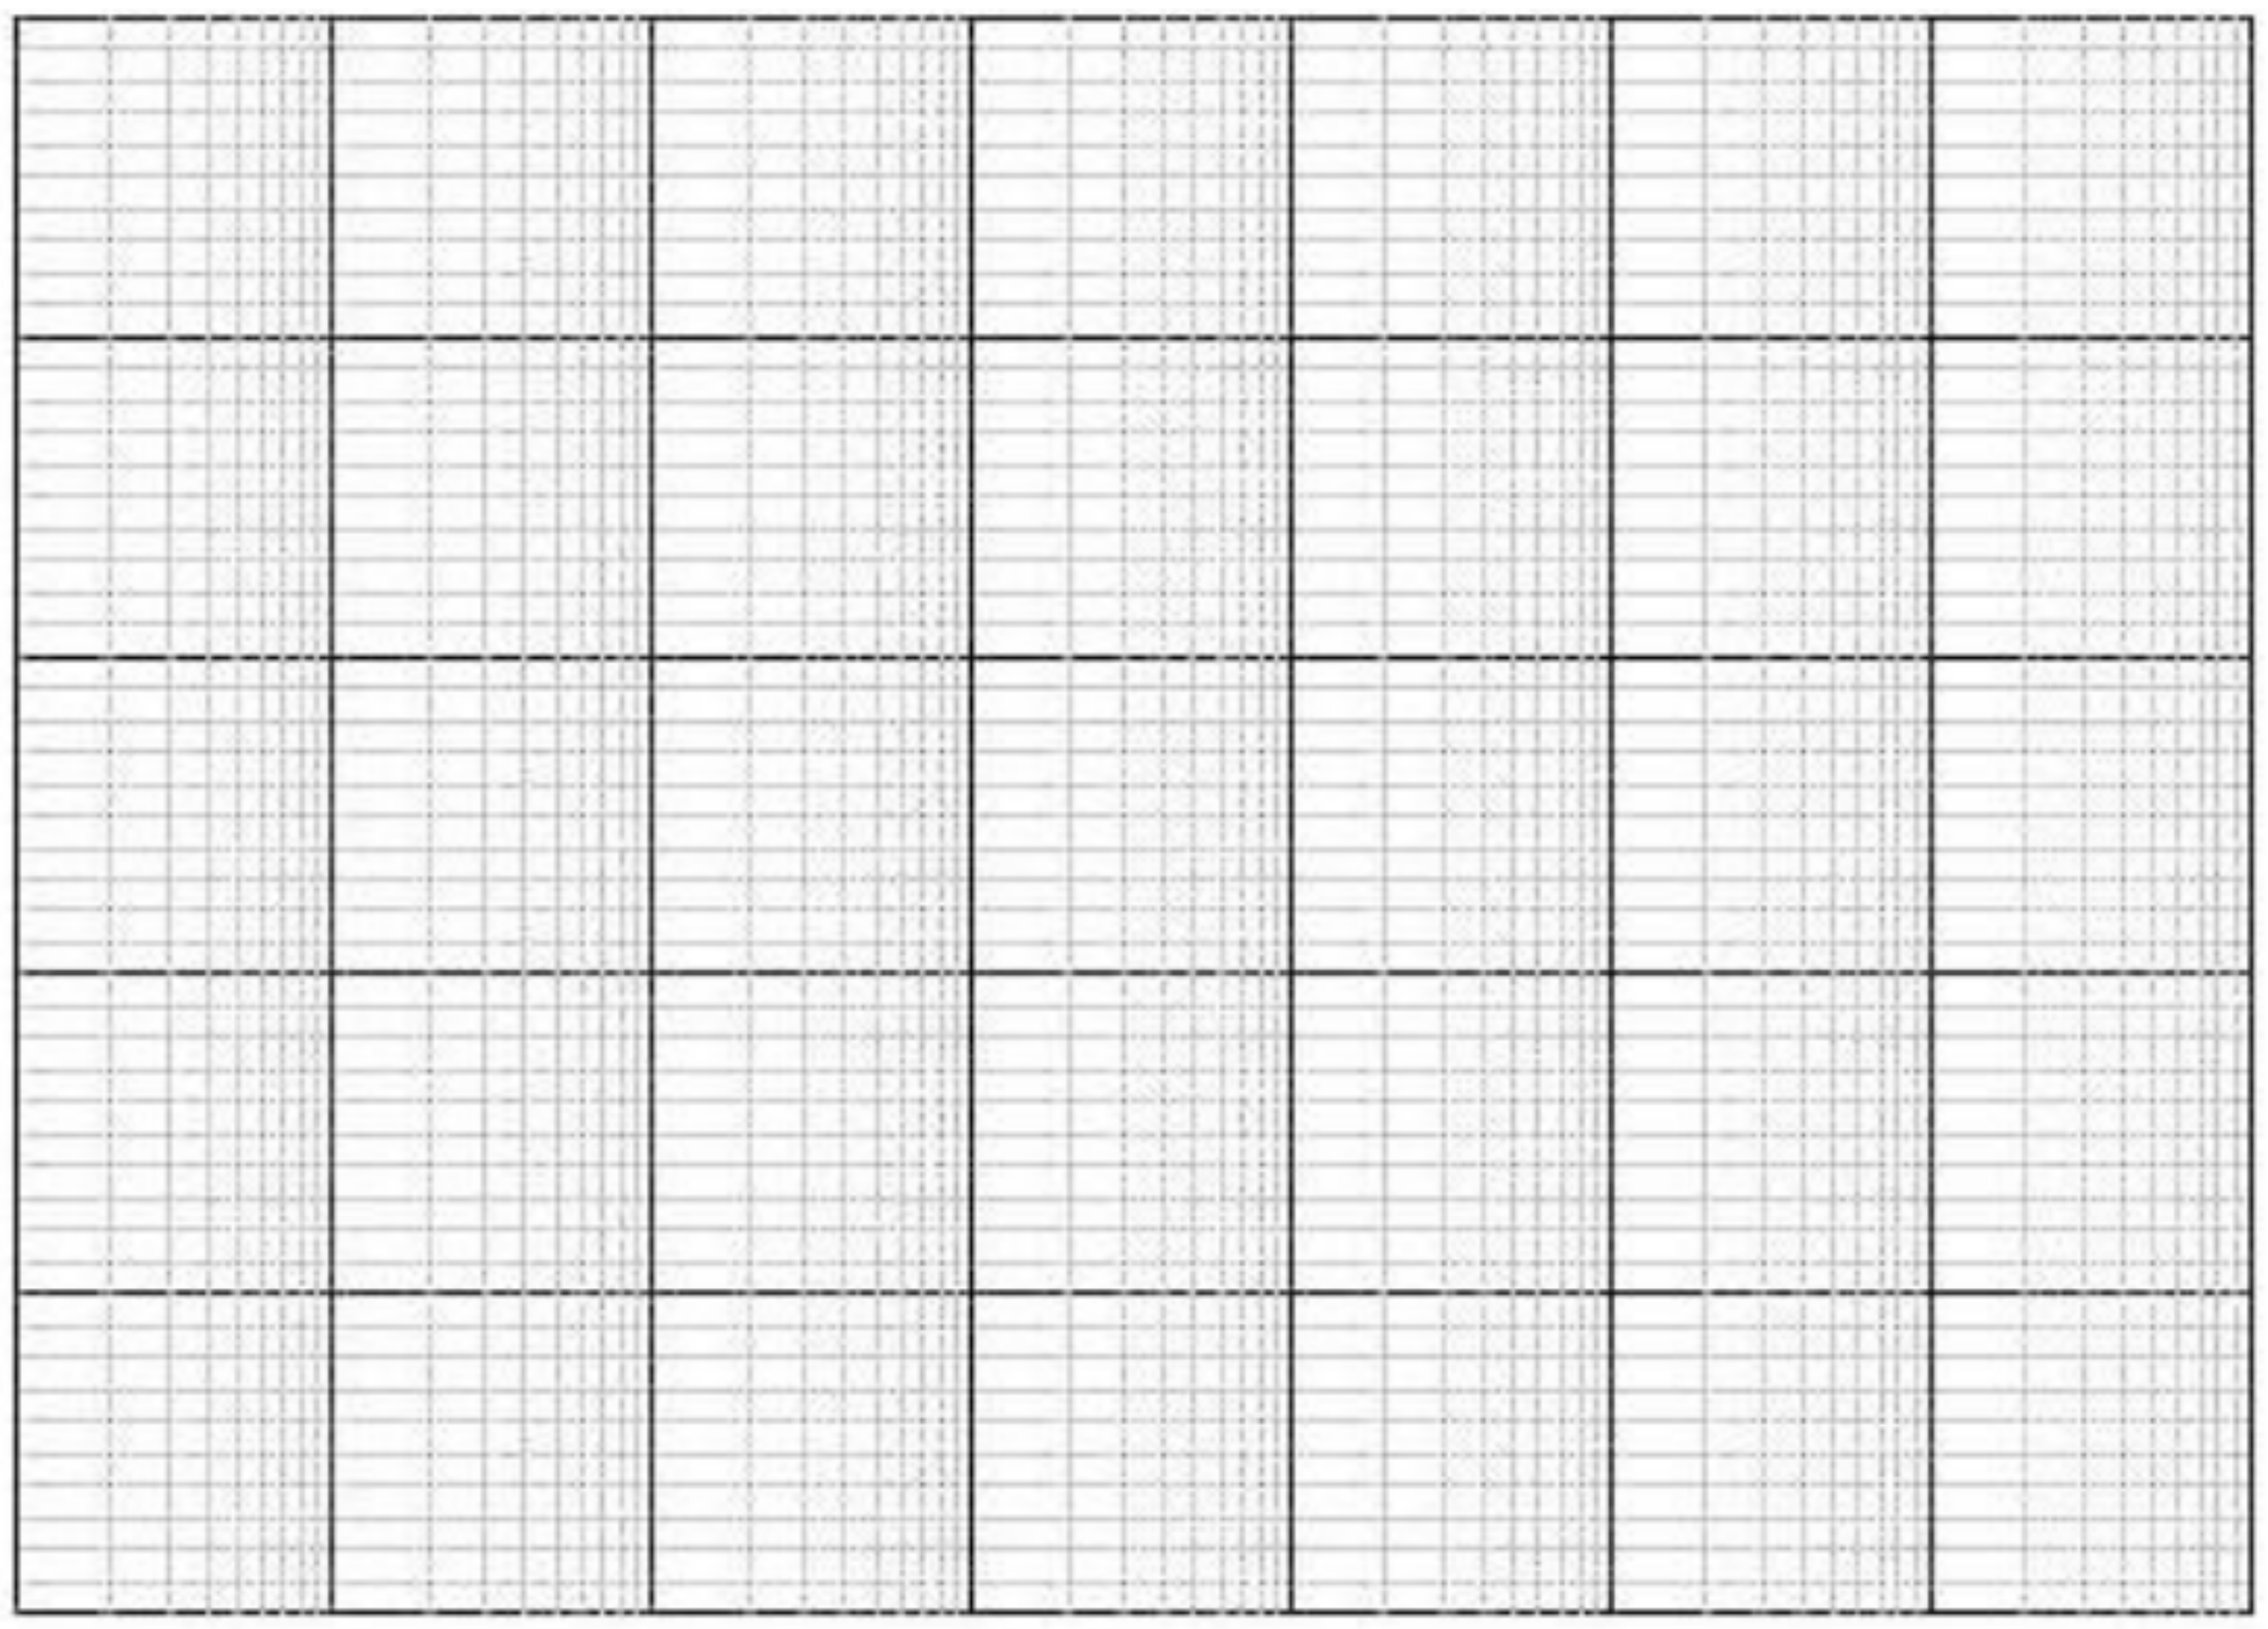
\includegraphics[width=1.0\textwidth]{\bank/transfer/figures/bodeblank}
    \caption*{$\angle H_z(\omega)$}
  \end{minipage}
\end{figure}

\sol{
}

\qitem \textbf{What is the relationship between zero and poles (both graphically and algebraically)?}

\sol{

}

\qitem (Optional) Let $H_0(\omega) = j\omega$. This is called a \textbf{zero at the origin}.
\begin{enumerate}
  \qitem \textbf{Find $|H_0(\omega)|$ and $\angle H_0(\omega)$}.
  \qitem \textbf{Sketch them on the next page.}

\begin{figure}[!h]
  \centering
  \begin{minipage}[b]{0.45\textwidth}
  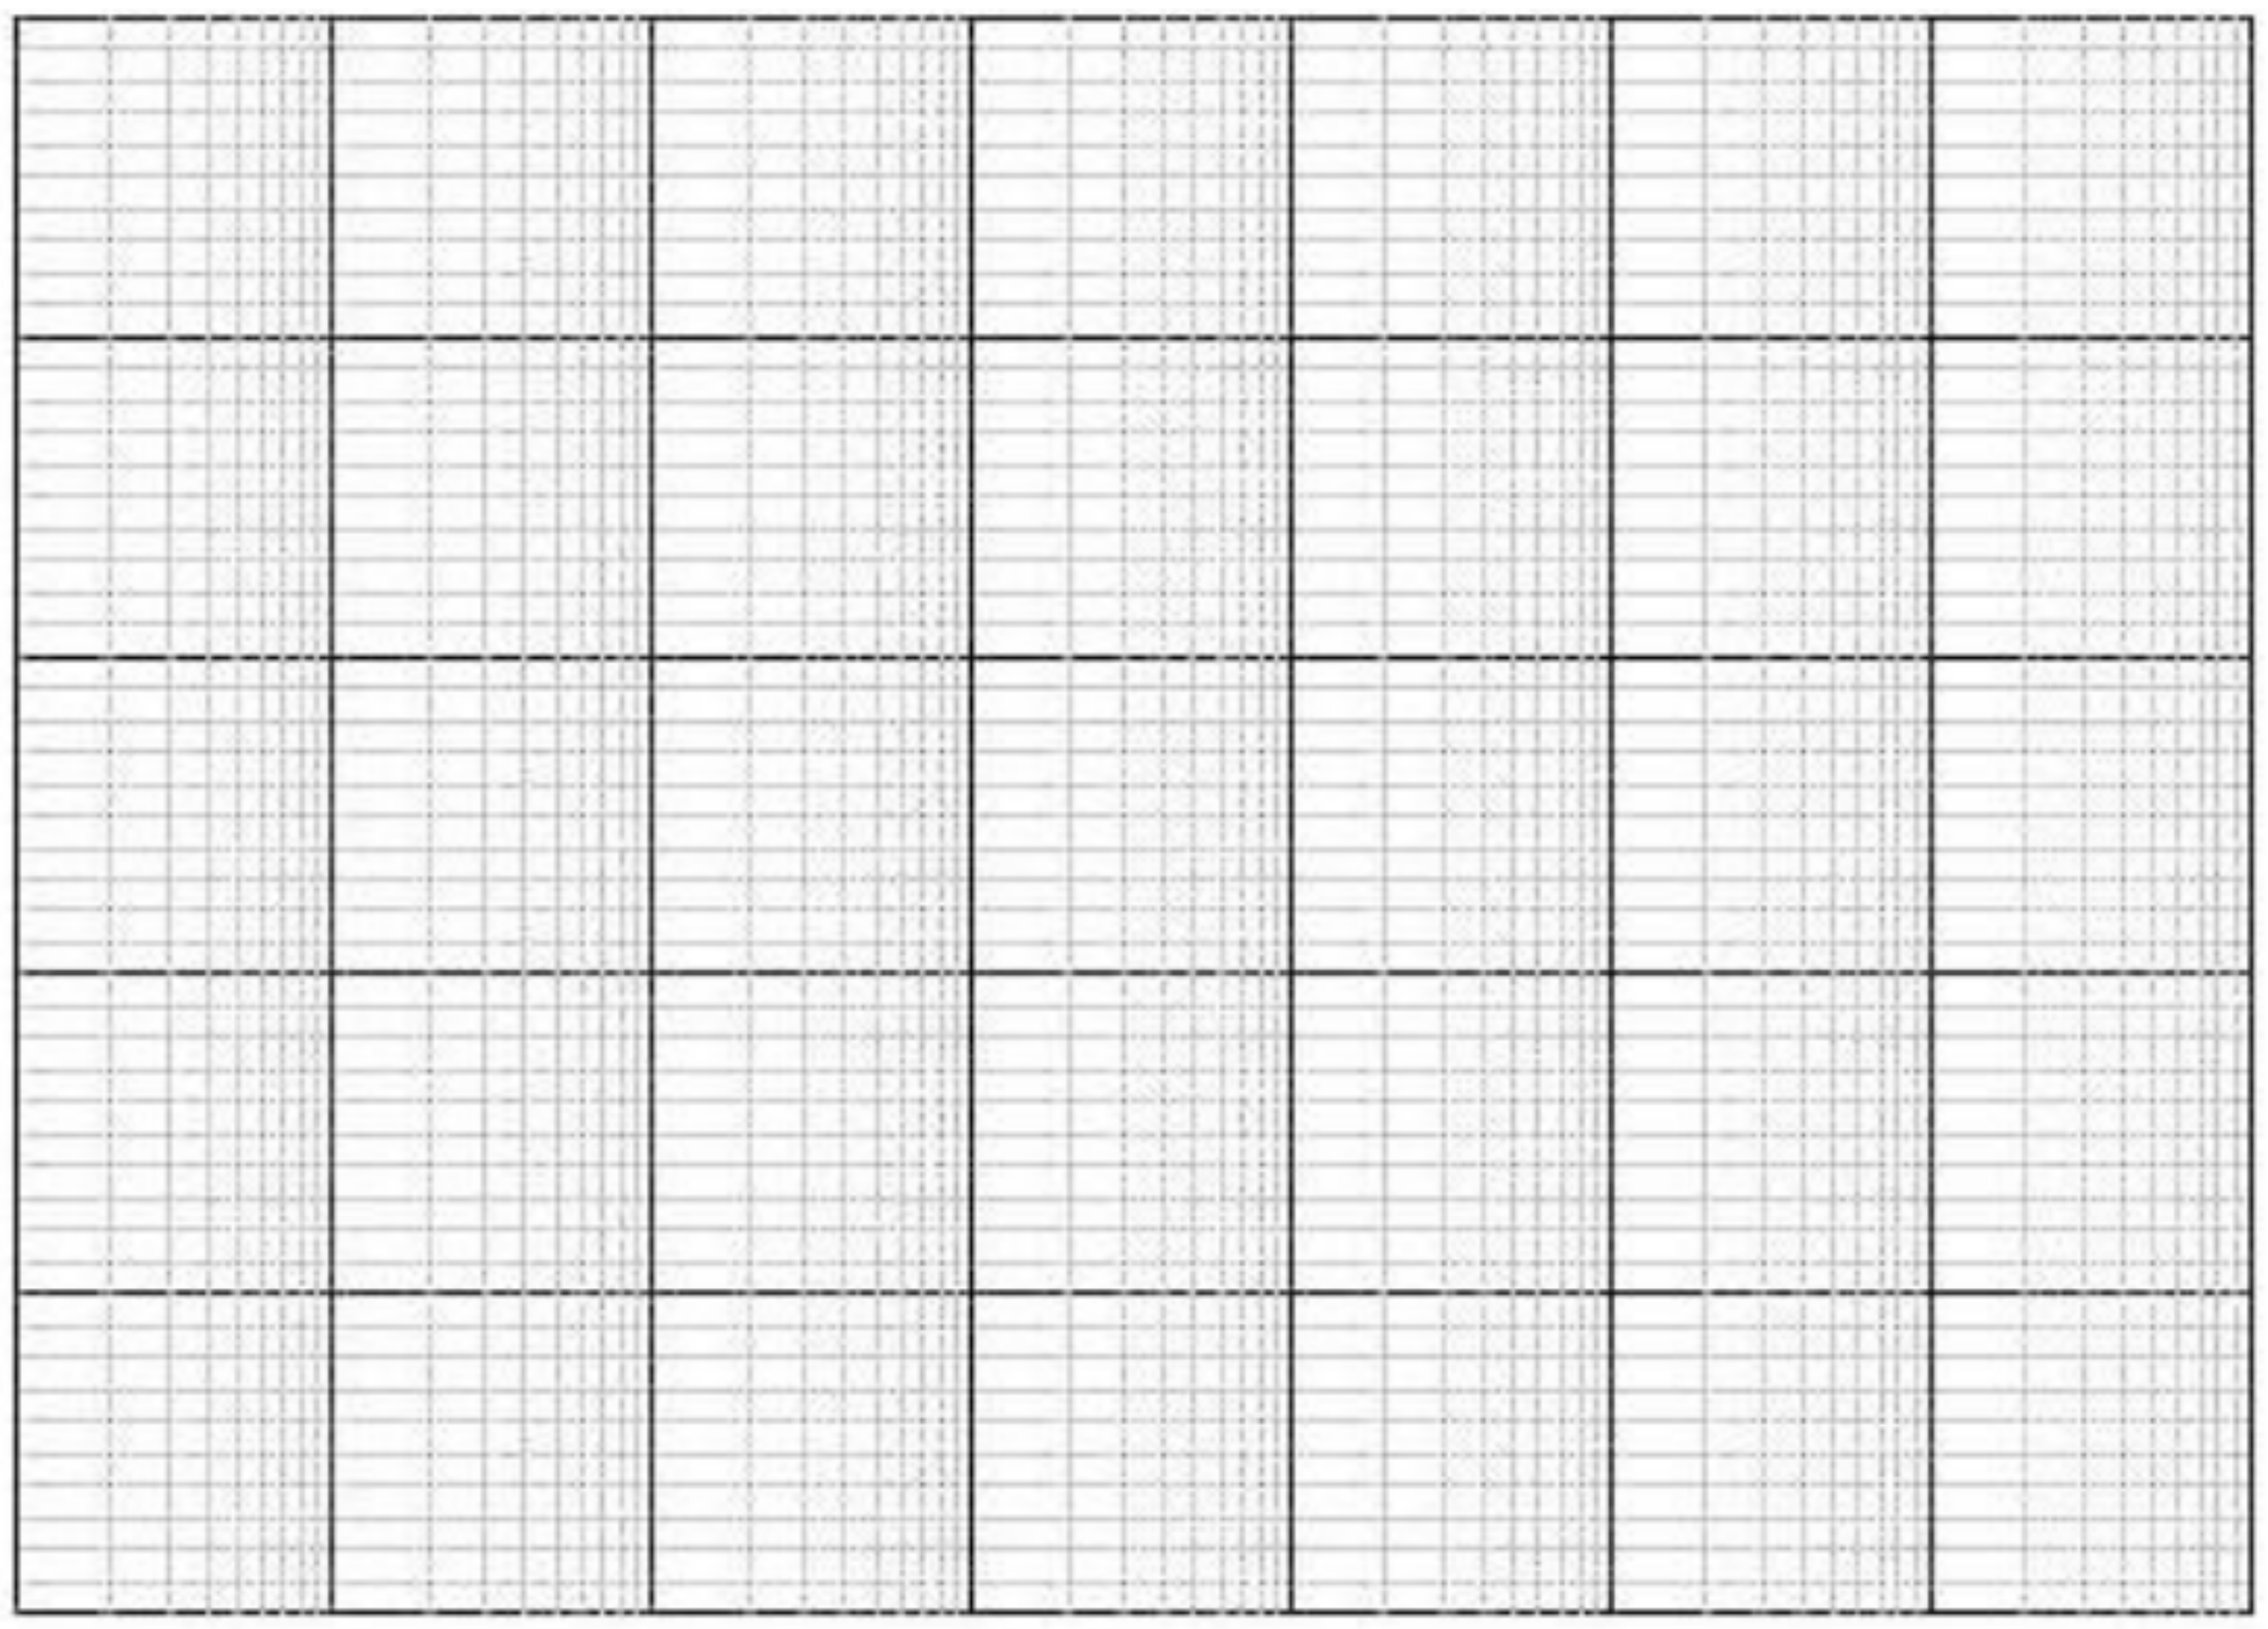
\includegraphics[width=1.0\textwidth]{\bank/transfer/figures/bodeblank}
    \caption*{$|H_0(\omega)|$}
  \end{minipage}
  \hfill
  \begin{minipage}[b]{0.45\textwidth}
  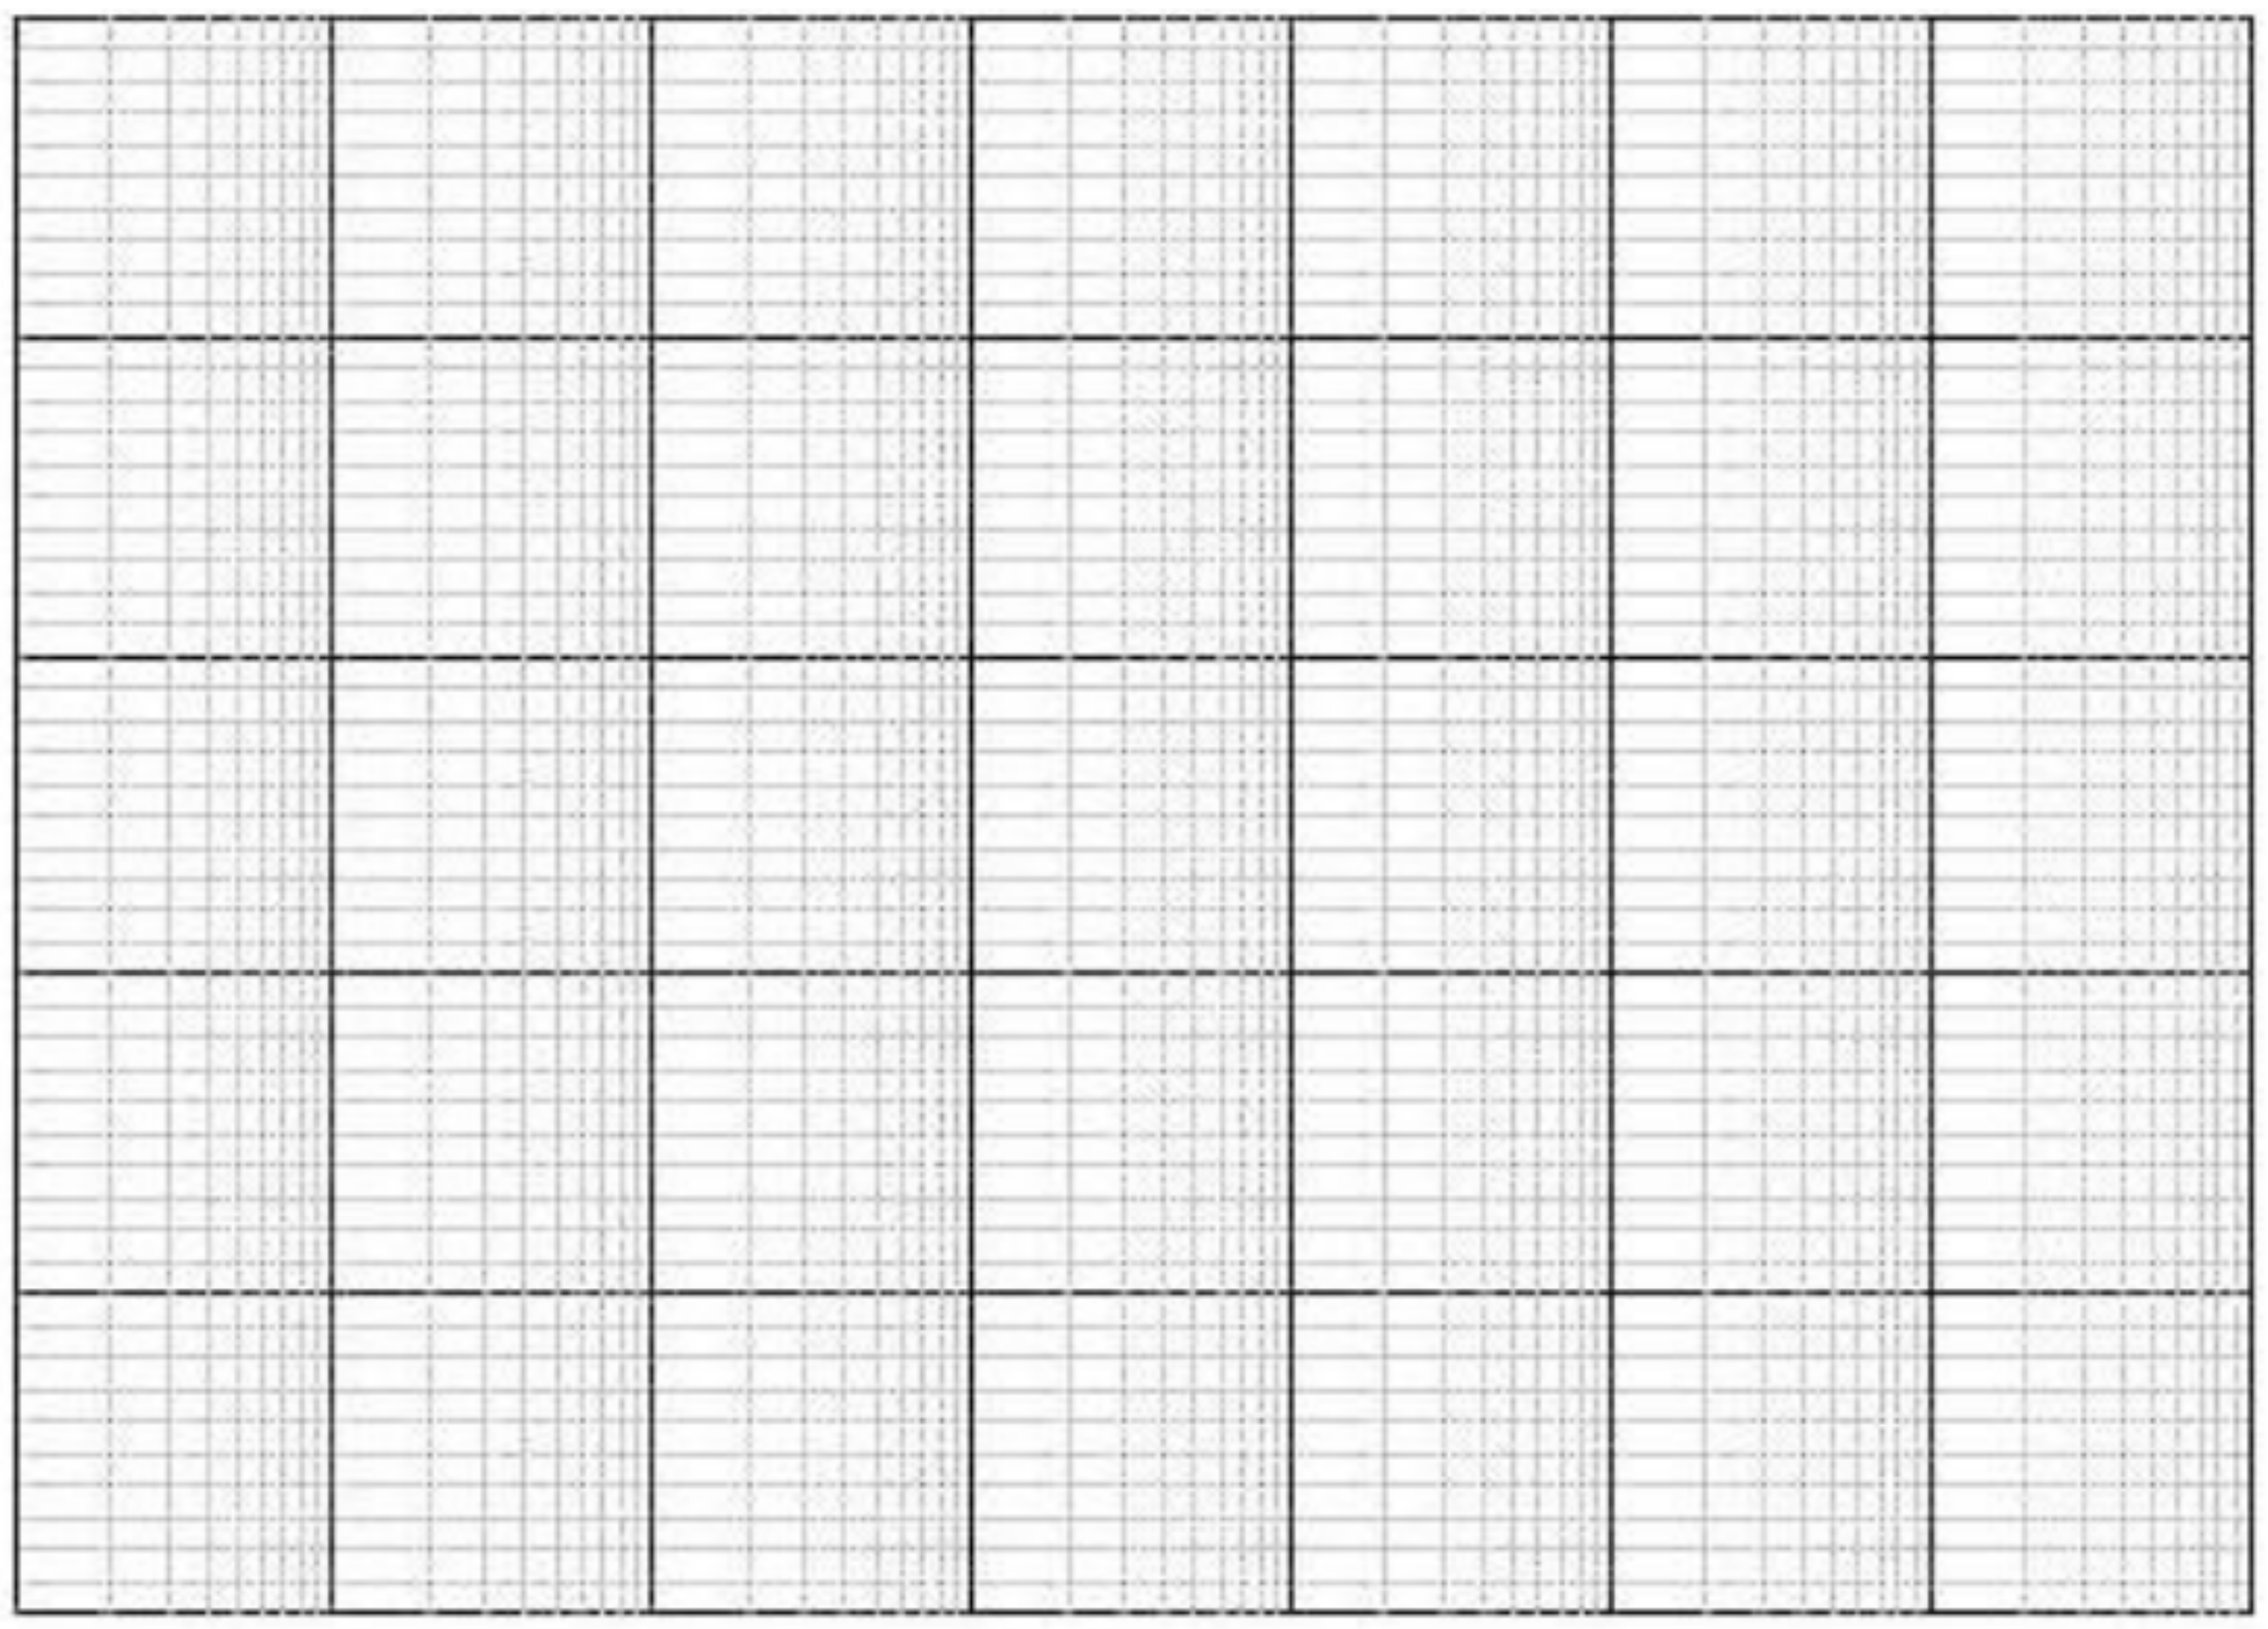
\includegraphics[width=1.0\textwidth]{\bank/transfer/figures/bodeblank}
    \caption*{$\angle H_0(\omega)$}
  \end{minipage}
\end{figure}
\end{enumerate}

\sol{
}

\qitem (Optional) Let $H_1(\omega) = \frac{1}{j\omega}$. This is called a \textbf{pole at the origin}.
\begin{enumerate}
  \qitem \textbf{Find $|H_1(\omega)|$ and $\angle H_1(\omega)$}. What are these in terms of $|H_0(\omega)|$ and $\angle H_0(\omega)$?
  \qitem \textbf{Sketch $|H_1(\omega)|$ and $\angle H_1(\omega)$ on the next page.}
\end{enumerate}

\begin{figure}[!h]
  \centering
  \begin{minipage}[b]{0.45\textwidth}
  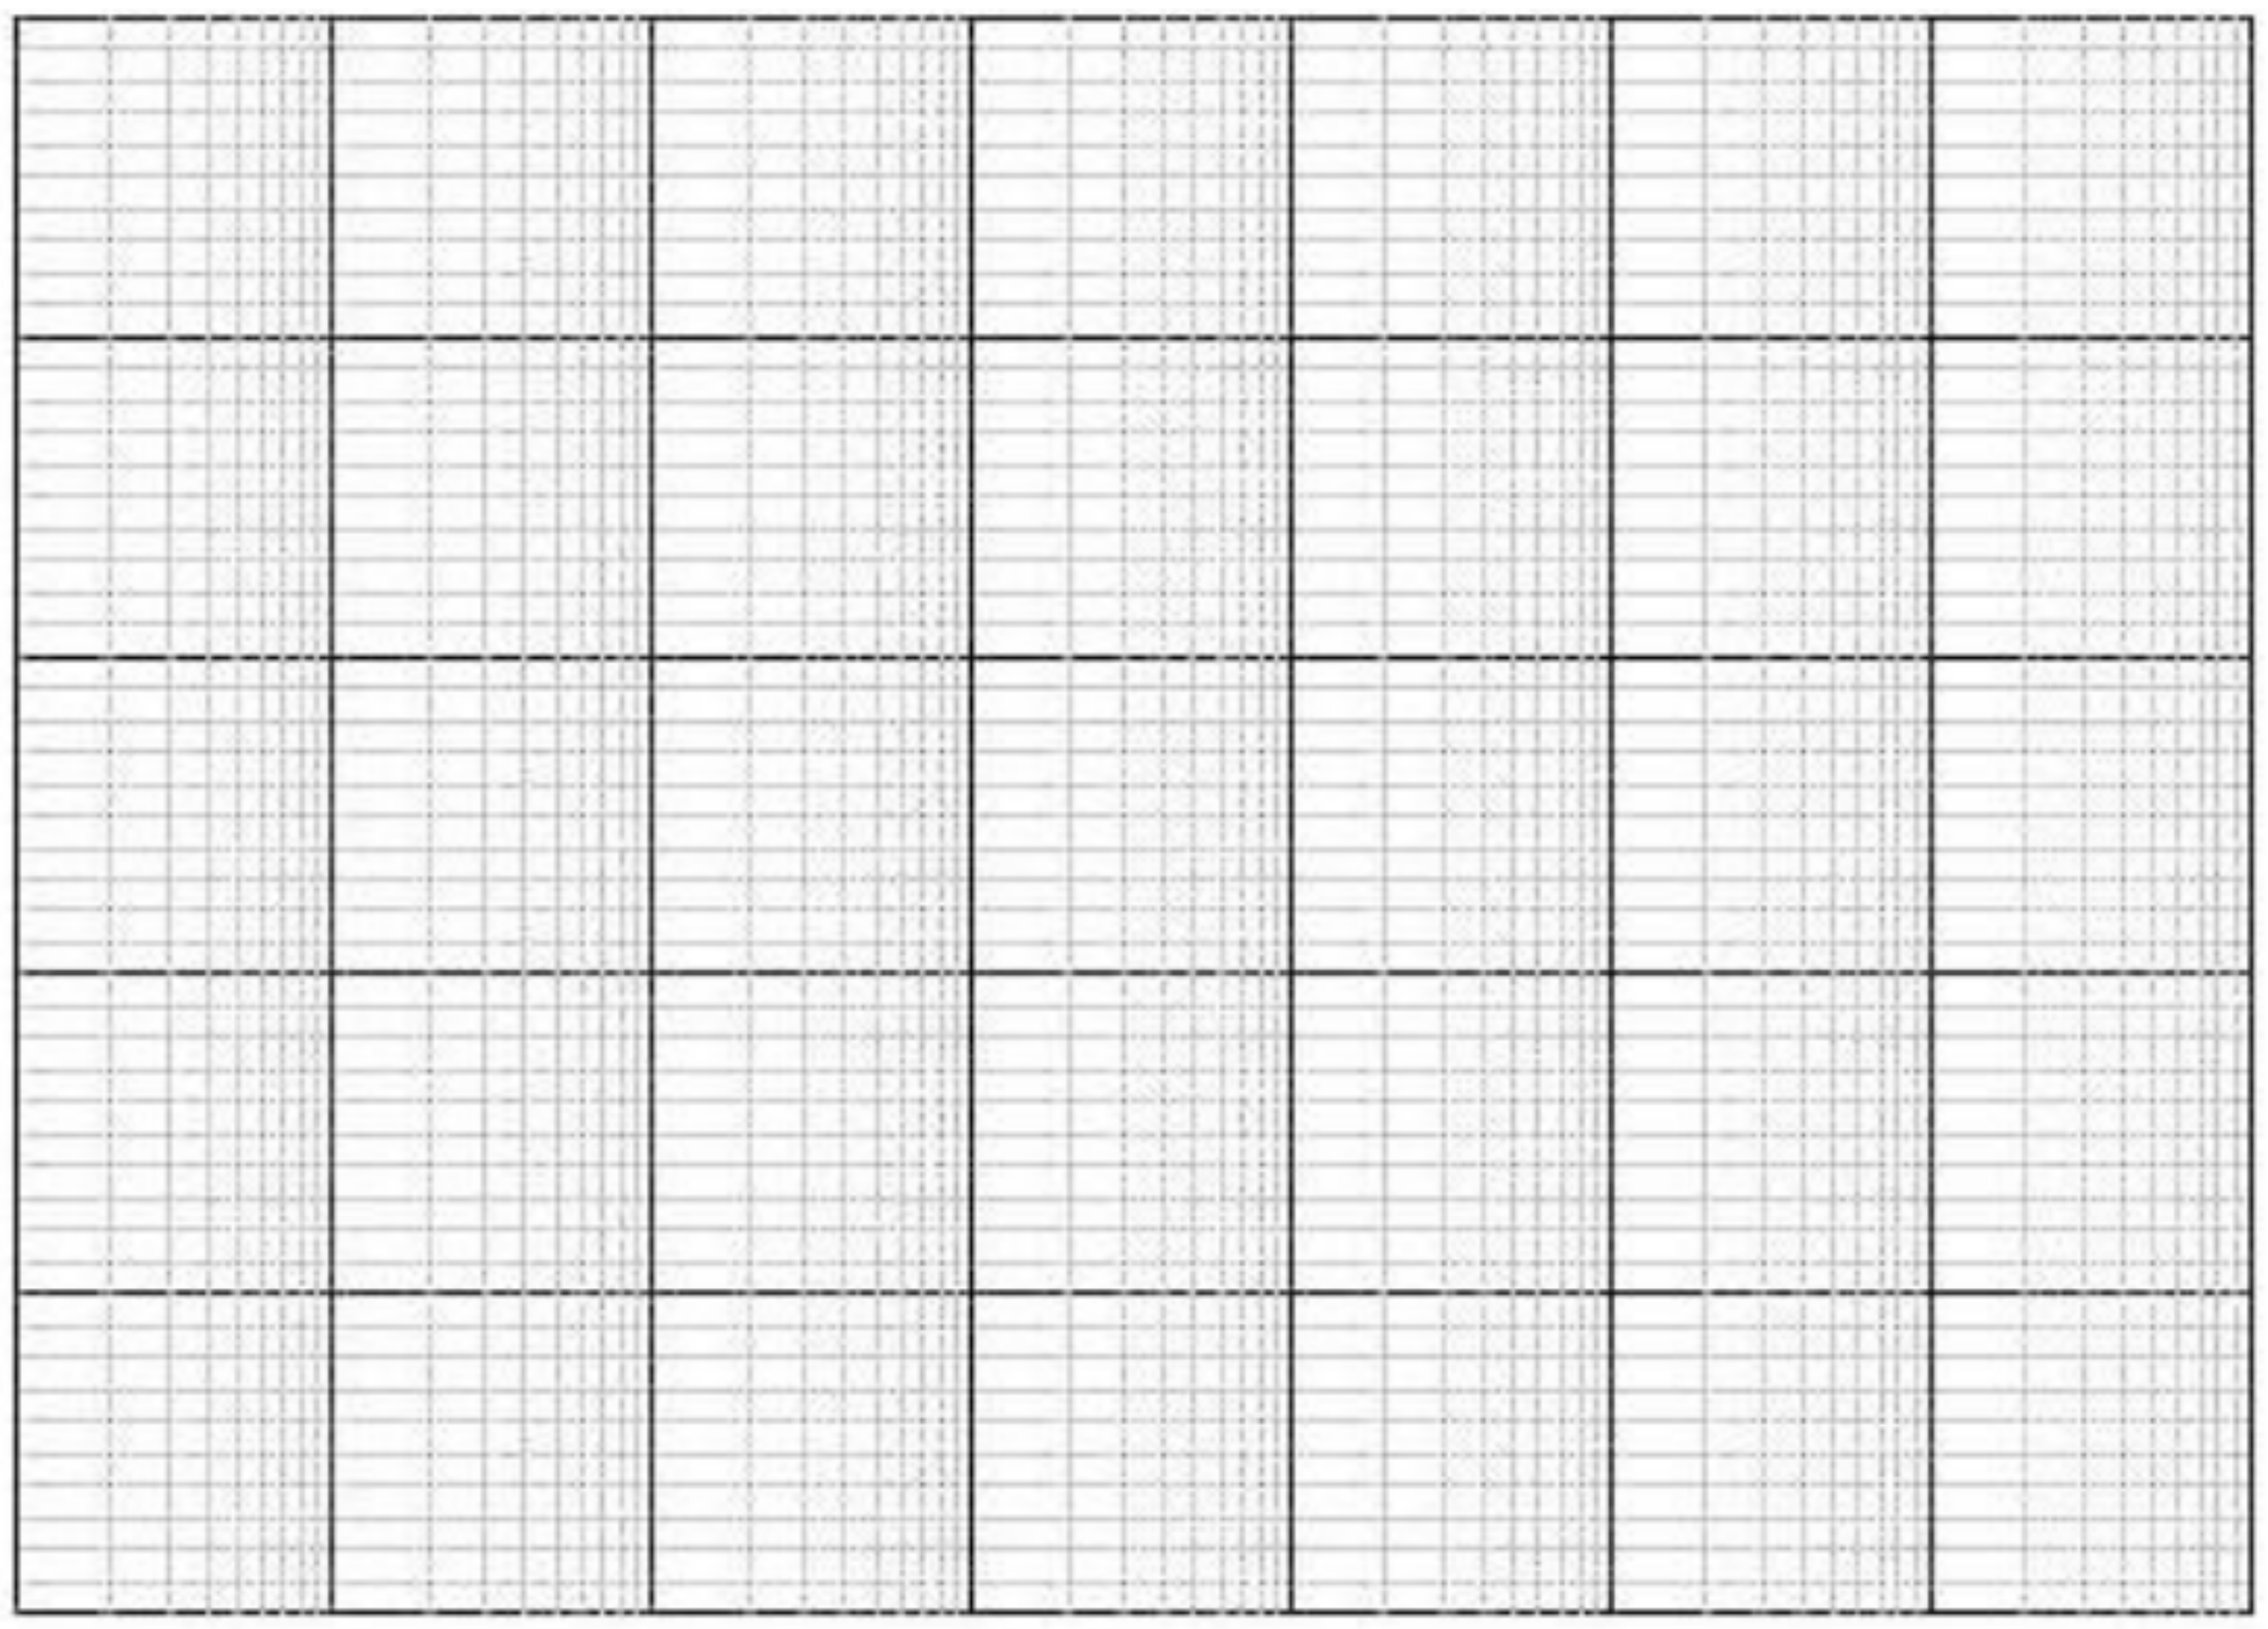
\includegraphics[width=1.0\textwidth]{\bank/transfer/figures/bodeblank}
    \caption*{$|H_1(\omega)|$}
  \end{minipage}
  \hfill
  \begin{minipage}[b]{0.45\textwidth}
  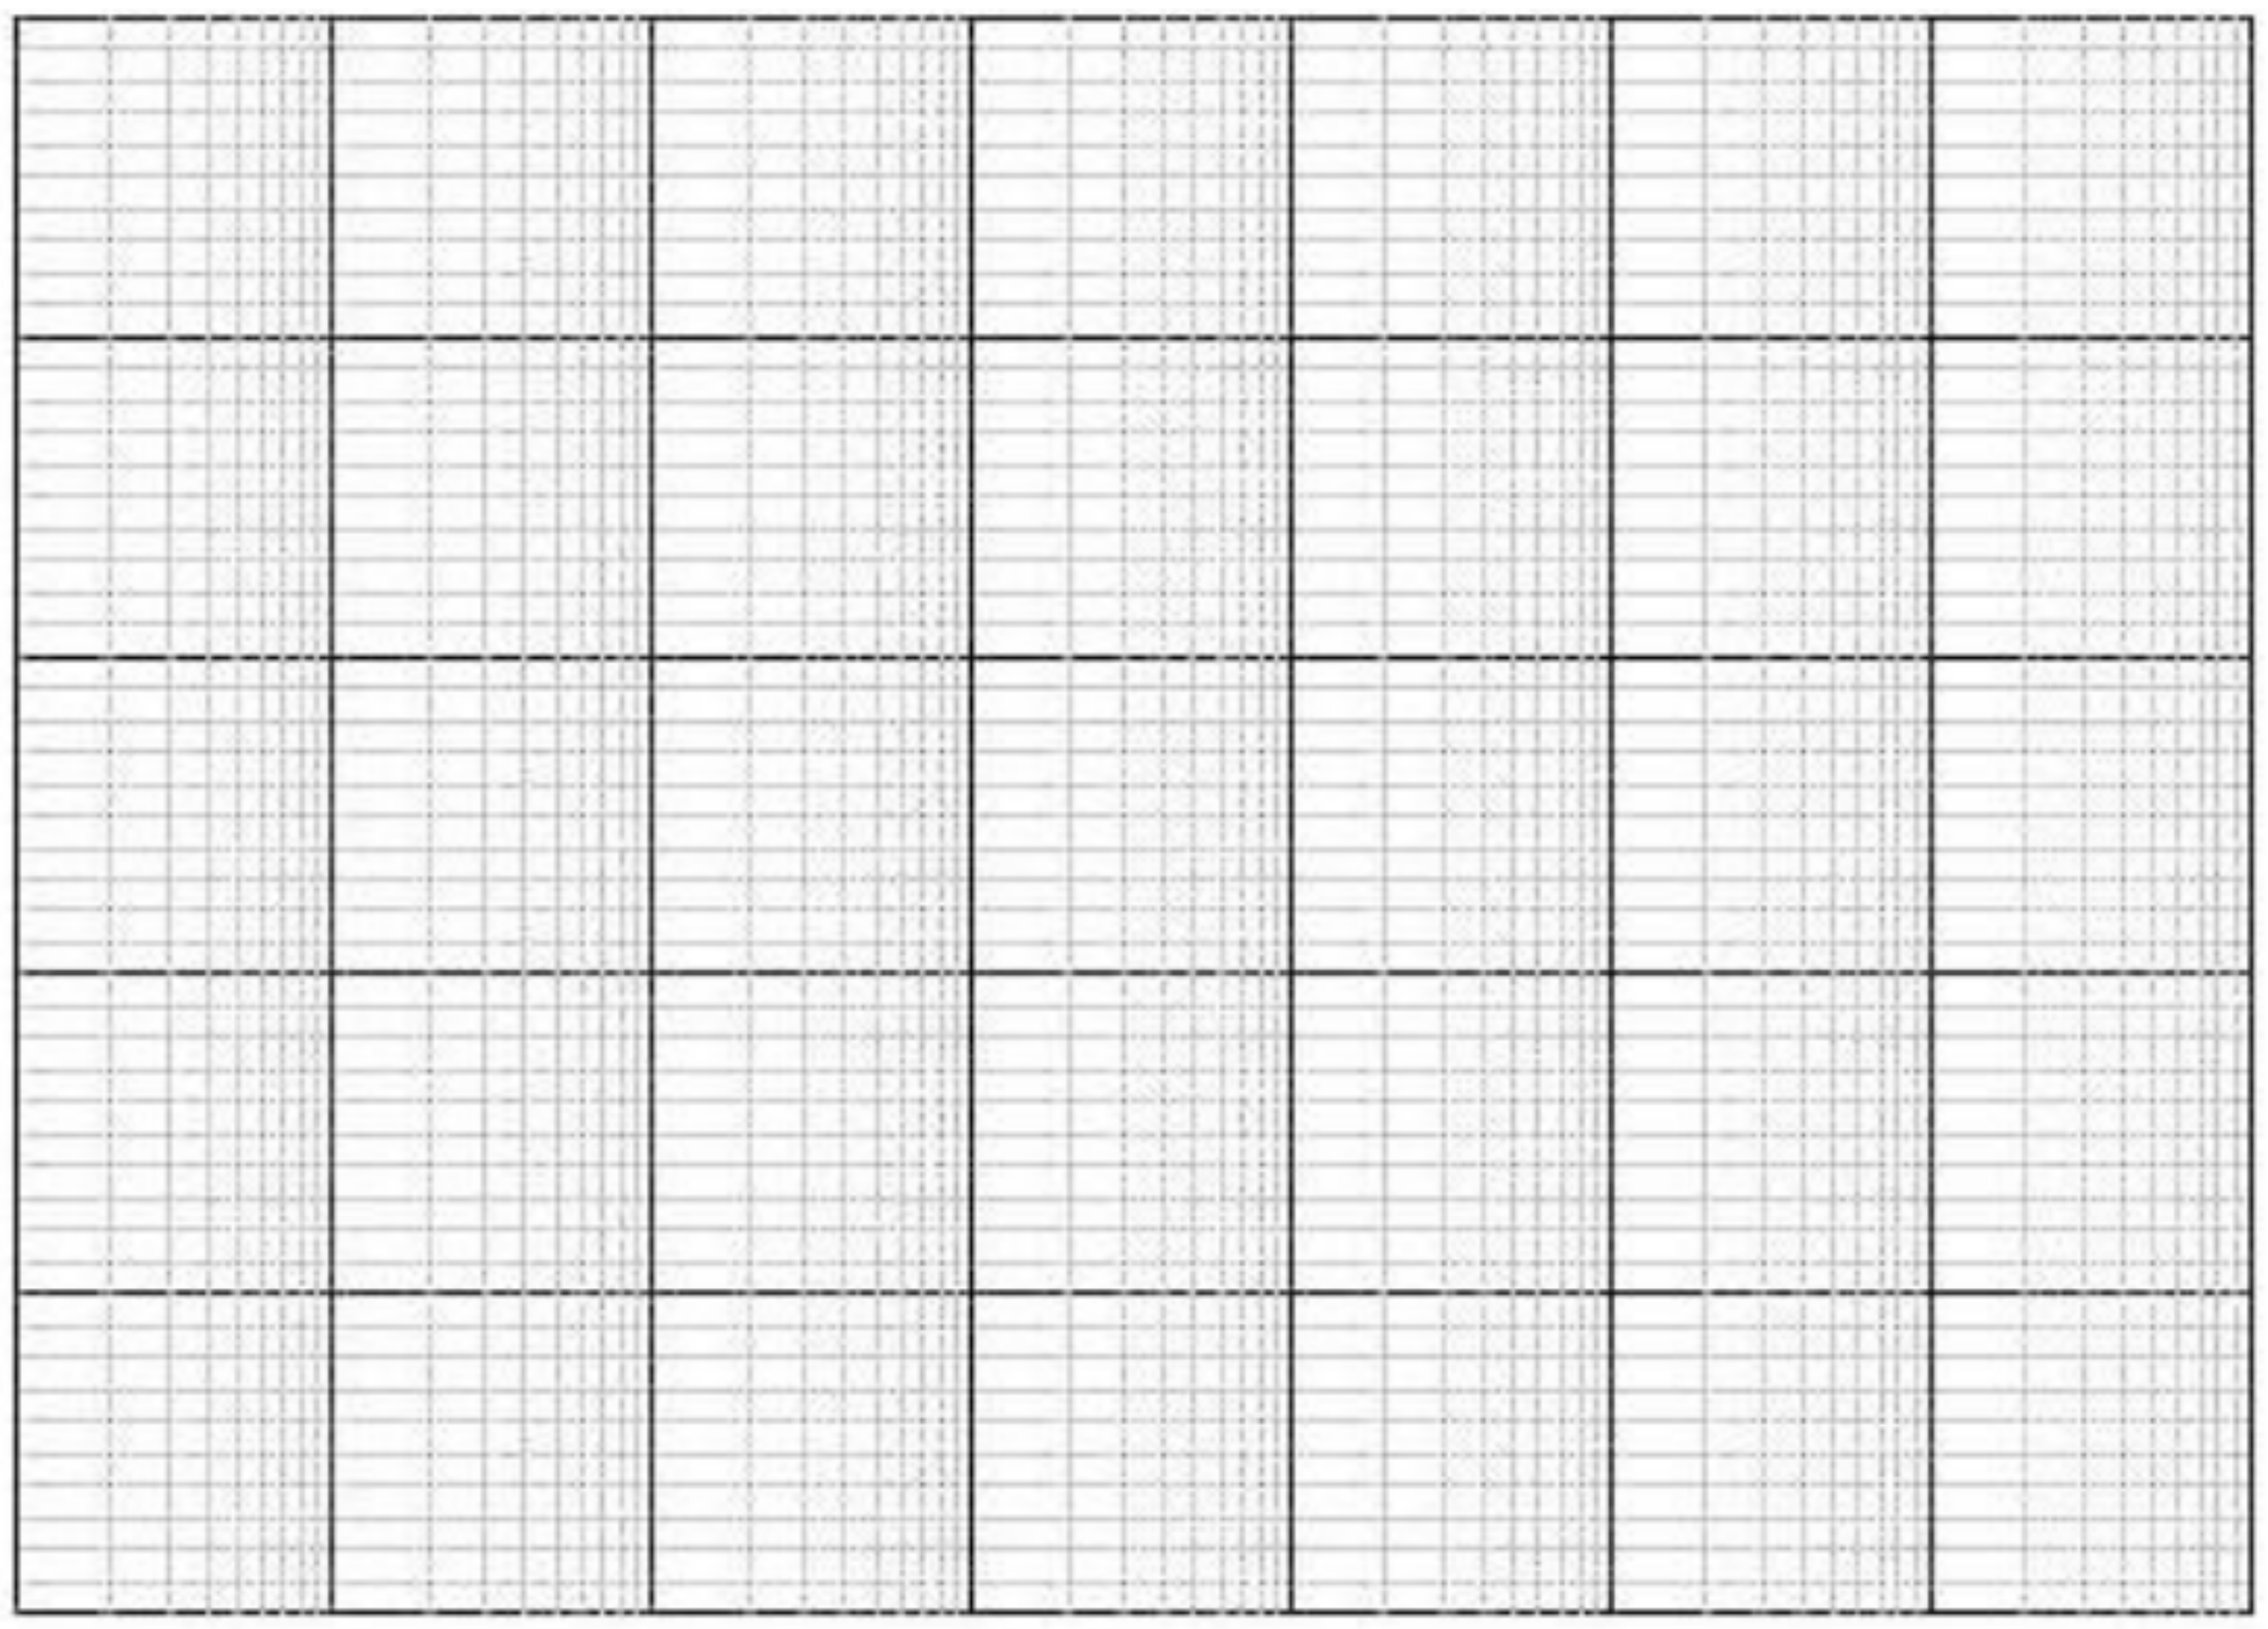
\includegraphics[width=1.0\textwidth]{\bank/transfer/figures/bodeblank}
    \caption*{$\angle H_1(\omega)$}
  \end{minipage}
\end{figure}

\sol{
}

\end{enumerate}
